%%%%%%%%%%%%%%%%%%%%%%%%%%%%%%%%%%%%%%%%%%%%%%%%%%%%%%%%%%%%%%%%%%%
%                                                                 %
%  GEANT manual in LaTeX form                              %
%                                                                 %
%  Michel Goossens (for translation into LaTeX)                   %
%  Version 1.00                                                   %
%  Last Mod. Jan 24 1991  1300   MG + IB                          %
%                                                                 %
%%%%%%%%%%%%%%%%%%%%%%%%%%%%%%%%%%%%%%%%%%%%%%%%%%%%%%%%%%%%%%%%%%%
\Origin{R.Brun, P.Zanarini}
\Submitted{15.11 83}     \Revised{13.12.93}
\Version{Geant 3.16}\Routid{DRAW399}
\Makehead{The data structure JDRAW}

This data structure contains the so-called \emph{view banks}. The
layout of the data structure can be found in Fig.~\ref{fg:draw399-1}.
The meaning of the variables is the following:
 
\begin{DLtt}{MMMMMMMM}
\item[NKVIEW]    number of views stored in the structure;
\item[IVIEW]     current view selected;
\item[IGU]       current graphic unit pointer;
\item[MAXGU]     number of units in graphic unit bank;
\item[MORGU]     number of words to push the graphic unit bank;
\item[IGS]       current graphic segment pointer;
\item[MAXGS]     number of segments in graphic segment bank;
\item[MORGS]     number of words to push the graphic segment bank;
\item[ITU]       current text unit pointer;
\item[MAXTU]     number of units in text unit bank;
\item[MORTU]     number of words to push the text unit bank;
\item[ITS]       current text segment pointer;
\item[MAXTS]     number of segments in text segment bank;
\item[MORTS]     number of words to push in text segment bank
\item[LENGU]     array of lengths for each graphic unit and of line attributes
({\tt LINATT});
\item[ADDGU]     array of addresses for each graphic unit;
\item[ADDTU]     array of addresses for each text unit;
\item[X]         array of u coordinates of graphic segments;
\item[Y]         array  v  coordinates of graphic segments;
\item[ICUT]      cut axis (1, 2, 3 or 0 if no cut) of the view;
\item[LINWID]    text line width and text attributes ({\tt ITXATT});
\end{DLtt}
{\tt GTHETA, GPHI, GPSI, GU0, GV0, GSCU, GSCV,} are the viewing
parameters stored in \FCind{/GCDRAW/}.
 
{\tt U0, V0, SIZE, ANGLE, IOPT, ITEXT} have the same meaning
of those given as arguments to \Rind{GDRAWT} (or \Rind{HPLSOF}~\cite{bib-HPLOT}).
 
A control word is stored in {\tt Q(JDRAW+IVIEW)}, with the following
meaning:
\begin{DLtt}{MMMM}
\item[1]  empty bank (created by internal routines to avoid gaps) or
for deleted banks;
\item[2]  bank created by the user;
\item[3]  protected bank reserved for internal use: it cannot be deleted by 
the user.
\end{DLtt}
\begin{figure}[hbt]
     \centering
     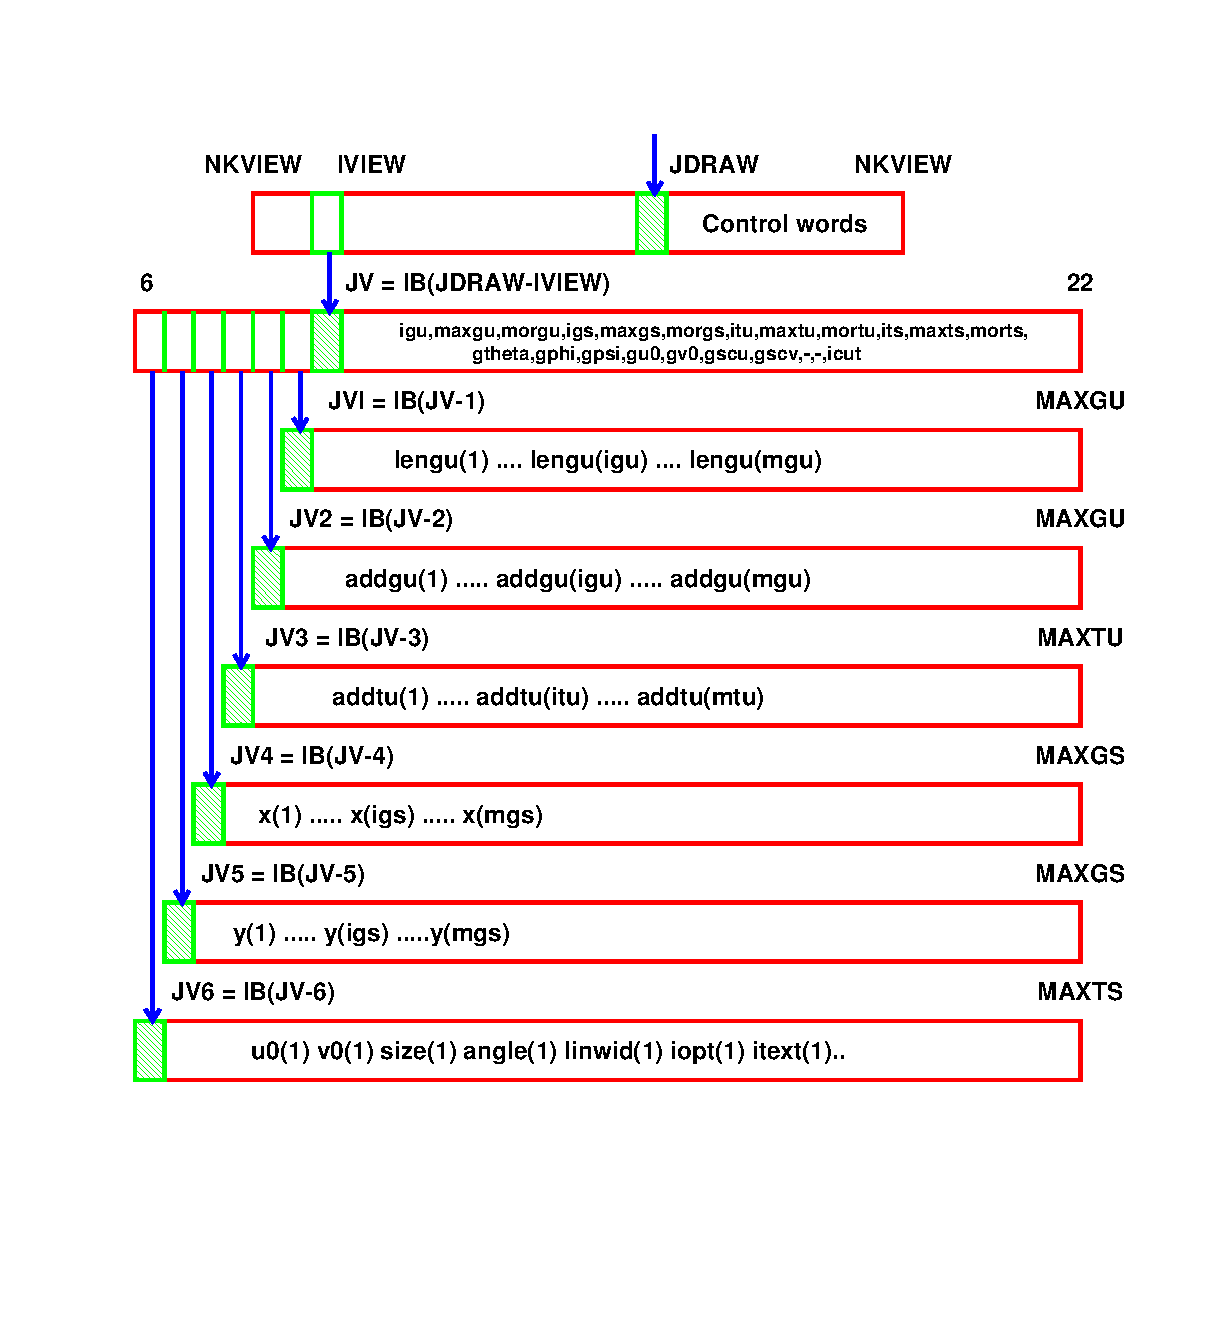
\epsfig{file=eps/draw399-1.eps,width=14cm}
     \caption{The {\tt JDRAW} data structure}
     \label{fg:draw399-1}
\end{figure}
